

\documentclass[crop, tikz]{standalone}
\usepackage{tikz}
\usepackage{amssymb}
\usetikzlibrary{calc}
\usepackage{colortbl}

 
% Definition of circles
\def\firstcircle{(0,0) circle (1.5cm)}
\def\secondcircle{(0:2cm) circle (1.5cm)}
\def\innercircle{(-0.3,0) circle (0.8cm)}

\colorlet{circle edge}{black!80}
\colorlet{circle area}{gray!50}

\tikzset{filled/.style={fill=circle area, draw=circle edge, thick},
    outline/.style={draw=circle edge, very thick}}

\setlength{\parskip}{5mm}
 
 \begin{document}

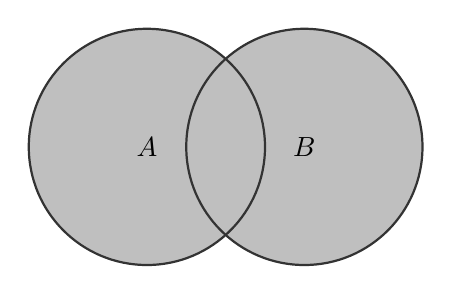
\begin{tikzpicture}
    \draw[filled] \firstcircle node {$A$}
                  \secondcircle node {$B$};
\end{tikzpicture}
 
\end{document}




 
